%% ============================================================ 1  MI 2025 P1 Q4
\defQ{1}{}{%
Three different blends of coffee beans -- Blend A, Blend B and Blend C -- are sold at both M Café and I Café. The usual selling prices of the blends are the same at both cafés. The total cost of buying one package each of Blend A, Blend B and Blend C is \$176. During a holiday sale the two cafés offered the following discounts:
\begin{center}\small
\begin{tabular}{|l|c|c|c|c|}\hline
\multirow{2}{*}{\textbf{Café}} & \multicolumn{3}{c|}{\textbf{Discounts given for each package}} & \textbf{Total price}\\\cline{2-4}
 & \textbf{Blend A} & \textbf{Blend B} & \textbf{Blend C} & \textbf{after the discount}\\\hline
\textbf{M Café} & 15\% & 10\% & 5\% & \$161.80\\\hline
\textbf{I Café} & 7\% & 5\% & 2\% & \$169.56\\\hline
\end{tabular}\end{center}
\begin{qparts}
\pt{(i)} Find the usual selling price of each package of Blend A, Blend B and Blend C coffee beans respectively. \mk{3}
\end{qparts}
\src{MI 2025 Prelim P1 Q4}}
\defS{1}{%
\begin{qparts}
\pt{(i)} Let the usual prices be $\$a$, $\$b$, $\$c$.
\begin{topalign}
a+b+c&=176 &&---(1)\\
0.85a+0.90b+0.95c&=161.80 &&---(2)\\
0.93a+0.95b+0.98c&=169.56 &&---(3)
\end{topalign}
$\gcsys$\ $a=32,\ b=44,\ c=100$\par
$\therefore$ Blend A: \$32,\ Blend B: \$44,\ Blend C: \$100
\end{qparts}}
%% ============================================================ 3  HCI 2025 P1 Q2
\defQ{3}{}{%
A sequence of real numbers, $x_n$, satisfies the recurrence relation
\[x_{n+1}=a(-3)^{n}+bn^{2}+cx_{n},\ \text{for } n,a,b,c\in\mathbb{Z}\ \text{and}\ n\geqslant1.\]
Given that $x_1=1$, $x_2=-8$, $x_3=70$, and $x_4=-377$, find the values of $a$, $b$ and $c$. \mk{3}\par
Hence, find the values of $x_{10}$ and $x_{11}$. \mk{2}
\src{HCI 2025 Prelim P1 Q2}}
\defS{3}{%
\begin{topalign}
&n=1\\
x_2&=a(-3)^{1}+b(1)^{2}+cx_1\\
-8&=-3a+b+c &&---(1)\\
&n=2\\
x_3&=a(-3)^{2}+b(2)^{2}+cx_2\\
70&=9a+4b-8c &&---(2)\\
&n=3\\
x_4&=a(-3)^{3}+b(3)^{2}+cx_3\\
-377&=-27a+9b+70c &&---(3)
\end{topalign}
$\gcsys$\ $a=2,\ b=3,\ c=-5$
\begin{topalign}
x_{n+1}&=2(-3)^{n}+3n^{2}-5x_{n}
\end{topalign}
\par\noindent\begin{minipage}[c]{0.45\linewidth}
$\gcsys$
\begin{topalign}
x_{10}&=-7\,210\,868\\
x_{11}&=36\,172\,738
\end{topalign}
\end{minipage}\hfill\begin{minipage}[c]{0.52\linewidth}\centering
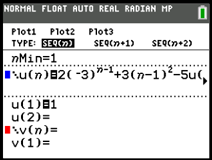
\includegraphics[width=0.48\linewidth]{gc/380863_lcd.png}\hfill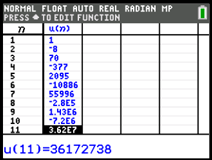
\includegraphics[width=0.48\linewidth]{gc/ce99e1_lcd.png}
\end{minipage}\par}
%% ============================================================ 4  SAJC 2025 P1 Q1
\defQ{4}{}{%
A function f is defined by $\mathrm{f}(x)=ax^{3}+bx^{2}+cx+d$ where $a$, $b$, $c$ and $d$ are constants. The graph of $y=\mathrm{f}(x)$ has a turning point at $x=-1$ and passes through the points $(2,10)$ and $(-2,-2)$. Given also that $\displaystyle\int_{-2}^{2}\mathrm{f}(x)\,\mathrm{d}x=16$, find the values of $a$, $b$, $c$ and $d$. \mk{4}
\src{SAJC 2025 Prelim P1 Q1}}
\defS{4}{%
\begin{topalign}
\mathrm{f}'(x)&=3ax^{2}+2bx+c\\
\mathrm{f}'(-1)&=0\\
3a-2b+c&=0 &&---(1)\\
\mathrm{f}(2)&=10\\
8a+4b+2c+d&=10 &&---(2)\\
\mathrm{f}(-2)&=-2\\
-8a+4b-2c+d&=-2 &&---(3)\\
\int_{-2}^{2}\big(ax^{3}+bx^{2}+cx+d\big)\,\mathrm{d}x&=16\\
\Big[\tfrac{a}{4}x^{4}+\tfrac{b}{3}x^{3}+\tfrac{c}{2}x^{2}+dx\Big]_{-2}^{2}&=16\\
(4a+\tfrac{8}{3}b+2c+2d)-(4a-\tfrac{8}{3}b+2c-2d)&=16\\
\tfrac{16}{3}b+4d&=16 &&---(4)
\end{topalign}
$\gcsys$\ $a=3,\ b=0,\ c=-9,\ d=4$}
%% ============================================================ 5  placeholder
\defQ{5}{}{%
The lines $l_{1}$ and $l_{2}$ have equations
\[\begin{aligned}
l_{1}:\ \mathbf{r}&=\begin{pmatrix}1\\2\\0\end{pmatrix}+\lambda\begin{pmatrix}-2\\1\\2\end{pmatrix},\\
l_{2}:\ \mathbf{r}&=\begin{pmatrix}0\\5\\-8\end{pmatrix}+\mu\begin{pmatrix}2\\-2\\3\end{pmatrix},
\end{aligned}\]
where $\lambda$ and $\mu$ are parameters.
\begin{qparts}
\pt{(i)} Show that $l_{1}$ and $l_{2}$ are skew lines. \mk{2}
\end{qparts}
\src{SAJC 2025 Prelim P1 Q3}}
\defS{5}{%
\begin{qparts}
\pt{(i)}
\begin{topalign}
1-2\lambda&=2\mu &&---(1)\\2+\lambda&=5-2\mu &&---(2)\\2\lambda&=-8+3\mu &&---(3)\\
\text{Solve (1) and (2): }\lambda&=-2,\ \mu=\tfrac52\\
&\text{Sub into (3):}\\
\text{LHS}&=2(-2)=-4\\
\text{RHS}&=-8+3\left(\tfrac52\right)=-\tfrac12\\
\text{LHS}&\neq\text{RHS},\ \text{no solution}\\
\therefore\ &l_{1}\text{ and }l_{2}\text{ do not intersect}\\
\because\ \begin{pmatrix}-2\\1\\2\end{pmatrix}&\neq k\begin{pmatrix}2\\-2\\3\end{pmatrix}\text{ for any } k\in\mathbb{R}\\
\therefore\ &l_{1}\text{ and }l_{2}\text{ are not parallel}\\
\therefore\ &l_{1}\text{ and }l_{2}\text{ are skew (shown)}
\end{topalign}
\end{qparts}}
%% ============================================================ 6  ACJC 2026 P1 Q1
\defQ{6}{}{%
Use an algebraic method to solve the inequalities
\[\frac{x(5x+9)}{x^{2}+2x+5}>x\geqslant3x-6.\] \mk{4}
\src{ACJC 2026 Prelim P1 Q1}}
\defS{6}{%
\begin{topalign}
x&\geqslant3x-6\\
x&\leqslant3 &&---(1)
\end{topalign}
\begin{topalign}
x^{2}+2x+5&=(x+1)^{2}+4>0\ \text{for all real } x
\end{topalign}
\begin{topalign}
\frac{x(5x+9)}{x^{2}+2x+5}&>x\\
5x^{2}+9x&>x(x^{2}+2x+5)\quad(\because x^{2}+2x+5>0)\\
x^{3}-3x^{2}-4x&<0\\
x(x-4)(x+1)&<0
\end{topalign}
\begin{center}\begin{tikzpicture}[x=1cm]
\draw[thin,-{Stealth[length=1.6mm]}](-3,0)--(3,0);
\foreach \p/\l in {-1.5/-1,0/0,1.5/4}{\draw(\p,0.1)--(\p,-0.1)node[below]{\small$\l$};}
\node at(-2.3,0.3){$-$};\node at(-0.75,0.3){$+$};\node at(0.75,0.3){$-$};\node at(2.3,0.3){$+$};
\end{tikzpicture}\end{center}
\begin{topalign}
x<-1\ \ \text{or}\ \ 0<x<4 &&---(2)
\end{topalign}
$(1)\cap(2):$\par
$\therefore\ x<-1\ \ \text{or}\ \ 0<x\leqslant3$}
%% ============================================================ 7  SAJC 2025 P2 Q1
\defQ{7}{}{%
\begin{qparts}
\pt{(i)} Solve the inequality $3\left|x^{2}-4\right|\leqslant\left|x+2\right|$. \mk{4}
\pt{(ii)} Hence, solve $\dfrac{3}{x^{2}}\left|1-4x^{2}\right|\leqslant\left|\dfrac{1+2x}{x}\right|$. \mk{2}
\end{qparts}
\src{SAJC 2025 Prelim P2 Q1}}
\defS{7}{%
\begin{qparts}
\pt{(i)} \begin{topalign}
3|x-2||x+2|&\leqslant|x+2|
\end{topalign}
$x=-2:\quad 0\leqslant0\ $ (true)\par
$x\neq-2:\ |x+2|>0$
\begin{topalign}
3|x-2|&\leqslant1\\
-\tfrac13\leqslant x-2&\leqslant\tfrac13\\
\tfrac53\leqslant x&\leqslant\tfrac73
\end{topalign}
$\therefore\ x=-2\ \ \text{or}\ \ \tfrac53\leqslant x\leqslant\tfrac73$
\pt{(ii)} \begin{topalign}
\frac{3}{x^{2}}\left|1-4x^{2}\right|&=3\left|\frac{1}{x^{2}}-4\right|\quad(\because x^{2}>0)\\
\left|\frac{1+2x}{x}\right|&=\left|\frac1x+2\right|\\
3\left|\Big(\frac1x\Big)^{2}-4\right|&\leqslant\left|\frac1x+2\right|\quad(x\to\tfrac1x)
\end{topalign}
\begin{topalign}
\frac1x=-2\ \ &\text{or}\ \ \frac53\leqslant\frac1x\leqslant\frac73
\end{topalign}
\begin{center}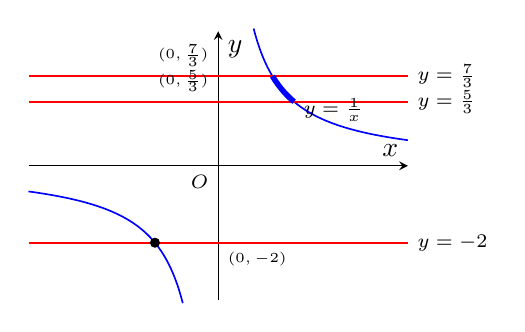
\begin{tikzpicture}
\begin{axis}[width=6.4cm,height=5cm,axis lines=middle,xmin=-1.5,xmax=1.5,ymin=-3.5,ymax=3.5,ticks=none,clip=false,xlabel=$x$,ylabel=$y$]
\addplot[blue,semithick,domain=0.28:1.5,samples=80]{1/x};
\addplot[blue,semithick,domain=-1.5:-0.28,samples=80]{1/x};
\addplot[red,semithick,domain=-1.5:1.5]{-2};\addplot[red,semithick,domain=-1.5:1.5]{5/3};\addplot[red,semithick,domain=-1.5:1.5]{7/3};\node[font=\scriptsize,anchor=north east] at (axis cs:0,0){$O$};\node[font=\tiny,anchor=north west] at (axis cs:0,-2){$(0,-2)$};\node[font=\tiny,anchor=south east] at (axis cs:0,5/3){$(0,\frac53)$};\node[font=\tiny,anchor=south east] at (axis cs:0,7/3){$(0,\frac73)$};
\addplot[blue,line width=2pt,domain=3/7:3/5]{1/x};\addplot[black,only marks,mark=*,mark size=1.6pt] coordinates{(-0.5,-2)};
\node[font=\scriptsize,anchor=west] at (axis cs:1.5,-2){$y=-2$};\node[font=\scriptsize,anchor=west] at (axis cs:1.5,5/3){$y=\frac53$};\node[font=\scriptsize,anchor=west] at (axis cs:1.5,7/3){$y=\frac73$};
\node[font=\scriptsize,anchor=south west] at (axis cs:0.6,0.9){$y=\frac1x$};
\end{axis}\end{tikzpicture}\end{center}
$\therefore\ x=-\tfrac12\ \ \text{or}\ \ \tfrac37\leqslant x\leqslant\tfrac35$
\end{qparts}}
%% ============================================================ 8  RVHS 2026 P1 Q2
\defQ{8}{}{%
\begin{qparts}
\pt{(a)} Solve the inequality $\left|\e^{x}-2\right|>\dfrac{1}{x^{2}-1}$ using a graphical approach. \mk{3}
\pt{(b)} Without the use of a graphing calculator, solve the inequality $\dfrac{x+2}{x-1}\geqslant\dfrac{2}{x-3}$. \mk{3}
\end{qparts}
\src{RVHS 2026 Prelim P1 Q2}}
\defS{8}{%
\begin{qparts}
\pt{(a)} \begin{center}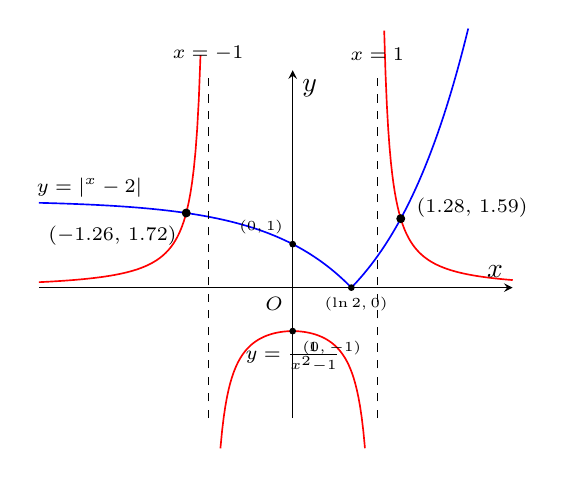
\begin{tikzpicture}
\begin{axis}[width=7.6cm,height=6cm,axis lines=middle,xmin=-3,xmax=2.6,ymin=-3,ymax=5,ticks=none,clip=false,xlabel=$x$,ylabel=$y$,restrict y to domain=-4:6]
\addplot[blue,semithick,domain=-3:2.1,samples=200]{abs(exp(x)-2)};
\addplot[red,semithick,domain=-3:-1.05,samples=100]{1/(x^2-1)};
\addplot[red,semithick,domain=-0.95:0.95,samples=100]{1/(x^2-1)};
\addplot[red,semithick,domain=1.05:2.6,samples=100]{1/(x^2-1)};\node[font=\scriptsize,anchor=north east] at (axis cs:0,0){$O$};\addplot[black,only marks,mark=*,mark size=1pt] coordinates{(0.6931,0)(0,1)(0,-1)};\node[font=\tiny,anchor=north] at (axis cs:0.75,0){$(\ln2,0)$};\node[font=\tiny,anchor=south east] at (axis cs:0,1){$(0,1)$};\node[font=\tiny,anchor=north west] at (axis cs:0,-1){$(0,-1)$};
\addplot[black,dashed,thin] coordinates{(-1,-3)(-1,5)};\addplot[black,dashed,thin] coordinates{(1,-3)(1,5)};
\addplot[black,only marks,mark=*,mark size=1.4pt] coordinates{(-1.258,1.716)(1.277,1.586)};
\node[font=\scriptsize,anchor=north east] at (axis cs:-1.258,1.65){$(-1.26,\,1.72)$};
\node[font=\scriptsize,anchor=south west] at (axis cs:1.35,1.4){$(1.28,\,1.59)$};
\node[font=\scriptsize] at (axis cs:-2.4,2.3){$y=|\e^{x}-2|$};
\node[font=\scriptsize] at (axis cs:0,-1.6){$y=\frac{1}{x^{2}-1}$};
\node[font=\scriptsize,anchor=south] at (axis cs:-1,5){$x=-1$};\node[font=\scriptsize,anchor=south] at (axis cs:1,5){$x=1$};
\end{axis}\end{tikzpicture}\end{center}
$\gcsys$\ intersections at $x=-1.2581$, $x=1.2770$\par
$\therefore\ x<-1.26\ \ \text{or}\ \ -1<x<1\ \ \text{or}\ \ x>1.28$
\pt{(b)} \begin{topalign}
\frac{x+2}{x-1}-\frac{2}{x-3}&\geqslant0\\
\frac{(x+2)(x-3)-2(x-1)}{(x-1)(x-3)}&\geqslant0\\
\frac{x^{2}-3x-4}{(x-1)(x-3)}&\geqslant0\\
\frac{(x-4)(x+1)}{(x-1)(x-3)}&\geqslant0
\end{topalign}
\begin{center}\begin{tikzpicture}[x=1cm]
\draw[thin,-{Stealth[length=1.6mm]}](-3.2,0)--(3.2,0);
\foreach \p/\l in {-1.8/-1,-0.6/1,0.6/3,1.8/4}{\draw(\p,0.1)--(\p,-0.1)node[below]{\small$\l$};}
\node at(-2.5,0.3){$+$};\node at(-1.2,0.3){$-$};\node at(0,0.3){$+$};\node at(1.2,0.3){$-$};\node at(2.5,0.3){$+$};
\end{tikzpicture}\end{center}
$\therefore\ x\leqslant-1\ \ \text{or}\ \ 1<x<3\ \ \text{or}\ \ x\geqslant4$
\end{qparts}}
%% ============================================================ 10  TJC 2022 P2 Q1
\defQ{10}{}{%
A movie theatre supports a charity event by providing discounted movie tickets at the following prices based on age group.
\begin{center}\renewcommand{\arraystretch}{1.15}
\begin{tabular}{|c|c|}\hline
Age group & Discounted ticket price\\\hline
$\leqslant12$ years & \$6\\\hline
13 to 49 years & \$9\\\hline
\begin{tabular}{@{}c@{}}$\geqslant50$ years\\(senior citizen)\end{tabular} & \$4\\\hline
\end{tabular}\end{center}
The event organiser plans to spend \$700 to sponsor 100 participants of which at least 35 of them are senior citizens. Find the possible number of participants for each age group. \mk{4}
\src{TJC 2022 Prelim P2 Q1}}
\defS{10}{%
Let $x$, $y$, $z$ be the number of participants aged $\leqslant12$, 13 to 49 and $\geqslant50$ years respectively.
\begin{topalign}
\left.\begin{aligned}x+y+z&=100 &&---(1)\\6x+9y+4z&=700 &&---(2)\end{aligned}\ \right\}&\ \Rightarrow\ \text{Using GC, } x=\tfrac{200}{3}-\tfrac53z,\ y=\tfrac{100}{3}+\tfrac23z\\
z&\geqslant35\\
\because\ x&\geqslant0\\
\tfrac{200}{3}-\tfrac53z&\geqslant0\\
z&\leqslant40\\
\therefore\ 35&\leqslant z\leqslant40
\end{topalign}
$x$, $y$, $z$ are non-negative integers. Using GC table:
\begin{topalign}
z=37&\Rightarrow x=5,\ y=58\\
z=40&\Rightarrow x=0,\ y=60\\
\therefore\ (x,y,z)&=(5,58,37)\ \text{or}\ (0,60,40)
\end{topalign}}
%% ============================================================ 11  SAJC 2019 P1 Q2
\defQ{11}{}{%
\begin{qparts}
\pt{(i)} On the same axes, sketch the curves with equations $y=\left|2x^{2}+6x+4\right|$ and $y=3-4x$, indicating any intercepts with the axes and points of intersection. Hence solve the inequality $3-4x<\left|2x^{2}+6x+4\right|$. \mk{4}
\pt{(ii)} Find the exact area bounded by the graphs of $y=3-4x$, $y=\left|2x^{2}+6x+4\right|$, $x=-3$ and $x=-1$. \mk{3}
\end{qparts}
\src{SAJC 2019 Prelim P1 Q2}}
\defS{11}{%
\begin{qparts}
\pt{(i)} \begin{center}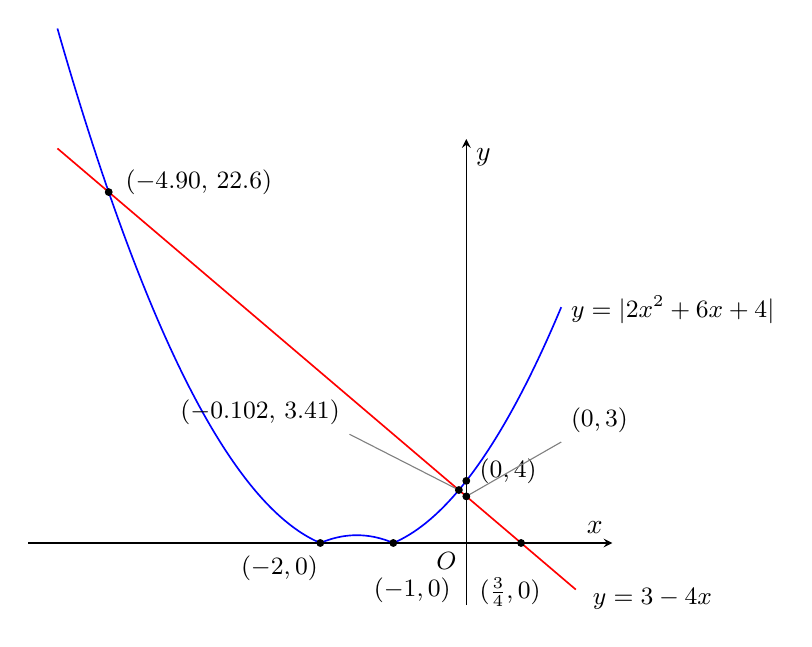
\begin{tikzpicture}
\begin{axis}[width=9cm,height=7.5cm,axis lines=middle,xmin=-6,xmax=2,ymin=-4,ymax=26,ticks=none,clip=false,xlabel=$x$,ylabel=$y$]
\addplot[blue,semithick,domain=-5.6:1.3,samples=300]{abs(2*x^2+6*x+4)};
\addplot[red,semithick,domain=-5.6:1.5]{3-4*x};
\addplot[black,only marks,mark=*,mark size=1.2pt] coordinates{(0,4)(0,3)(-2,0)(-1,0)(0.75,0)(-4.898,22.59)(-0.1021,3.408)};
\node[font=\small,anchor=north east] at (axis cs:0,0){$O$};
\node[font=\small,anchor=west] at (axis cs:0.05,4.6){$(0,4)$};
\draw[thin,gray] (axis cs:0,3)--(axis cs:1.3,6.5);\node[font=\small,anchor=south west] at (axis cs:1.3,6.5){$(0,3)$};
\node[font=\small,anchor=north east] at (axis cs:-1.9,-0.2){$(-2,0)$};
\node[font=\small,anchor=north west] at (axis cs:-1.4,-1.6){$(-1,0)$};
\node[font=\small,anchor=north] at (axis cs:0.6,-1.6){$(\frac34,0)$};
\node[font=\small,anchor=west] at (axis cs:-4.8,23.2){$(-4.90,\,22.6)$};
\draw[thin,gray] (axis cs:-0.1021,3.408)--(axis cs:-1.6,7);\node[font=\small,anchor=south east] at (axis cs:-1.6,7){$(-0.102,\,3.41)$};
\node[font=\small,anchor=west] at (axis cs:1.3,15){$y=|2x^{2}+6x+4|$};
\node[font=\small,anchor=west] at (axis cs:1.6,-3.6){$y=3-4x$};
\end{axis}\end{tikzpicture}\end{center}
\begin{topalign}
3-4x&=2x^{2}+6x+4\\
2x^{2}+10x+1&=0\\
x&=\frac{-5\pm\sqrt{23}}{2}\\
\therefore\ x&<\frac{-5-\sqrt{23}}{2}\ \ \text{or}\ \ x>\frac{-5+\sqrt{23}}{2}
\end{topalign}
\pt{(ii)}
\begin{topalign}
\text{Area}&=\int_{-3}^{-1}\left(3-4x-\left|2x^{2}+6x+4\right|\right)\mathrm{d}x\\
&=\int_{-3}^{-2}\left(3-4x-2x^{2}-6x-4\right)\mathrm{d}x+\int_{-2}^{-1}\left(3-4x+2x^{2}+6x+4\right)\mathrm{d}x\\
&=\int_{-3}^{-2}\left(-2x^{2}-10x-1\right)\mathrm{d}x+\int_{-2}^{-1}\left(2x^{2}+2x+7\right)\mathrm{d}x\\
&=\left[-\tfrac23x^{3}-5x^{2}-x\right]_{-3}^{-2}+\left[\tfrac23x^{3}+x^{2}+7x\right]_{-2}^{-1}\\
&=\left(\tfrac{16}{3}-20+2\right)-\left(18-45+3\right)+\left(-\tfrac23+1-7\right)-\left(-\tfrac{16}{3}+4-14\right)\\
&=20
\end{topalign}
\end{qparts}}
